\documentclass{article}
\usepackage{tikz}

\makeatletter
\newbox\@tempboxb
\def\gt#1{{\small\texttt{#1}}}
\def\args(#1,#2){% typeset the description of the arguments
\setbox\@tempboxa\hbox{\hspace{0.08\textwidth}\small\texttt{#1}}%
\ifdim \wd\@tempboxa>0.35\textwidth
\setbox\@tempboxb\hbox{#2}\ifdim\wd\@tempboxb>5pt
\hbox to0.95\textwidth{\begin{tabular}{p{0.38\textwidth}@{}p{0.6\textwidth}}
\hbox to 0.33\textwidth{\unhbox\@tempboxa\hss}&{}\\[-12pt]
{}&#2
\end{tabular}\hss}\par%
\else
\hbox to0.95\textwidth{\begin{tabular}{p{0.38\textwidth}@{}p{0.6\textwidth}}
\hbox to 0.33\textwidth{\unhbox\@tempboxa\hss}&{}
\end{tabular}\hss}\par\kern -12pt%
\fi
\else
\hbox to0.95\textwidth{\begin{tabular}{p{0.38\textwidth}@{}p{0.6\textwidth}}
\unhbox\@tempboxa{}&#2
\end{tabular}\hss}\par%
\fi
}
\makeatother
\hyphenation{turn-it-in}
\newenvironment{remark}{\smallskip\par\noindent\textbf{\large Remark}\par\smallskip\noindent\bgroup\ignorespaces}{\egroup}
\begin{document}
\title{How to use LTI services}
\author{Laszlo Csirmaz\\\small Central European University, Budapest}
\date{December 10, 2014}
\maketitle
\section{Introduction}\label{sec:intro}
Starting from the end of 2015, Turnitin plans to terminate support for the
legacy API interface, and offers its services as an LTI Tool Provider. In this
note we explain the basic model behind using those services (Section
\ref{sec:model}), discuss the connection between the old and new terminology
(Section \ref{sec:terminology}), and give examples for some
of the new calls (Section \ref{sec:lti-calls} and \ref{sec:soap-calls}). 

Material in this note was composed exclusively from publicly available 
information. The most important source was the Moodle integration module
by John McGettrick \cite{moodlev2}. The tutorial \cite{tutorial} explains
what parameters a Tool Provider should expect.

As always, there is no guarantee for 
the correctness of any information or statement in this note.

\section{The Learning Management System model}\label{sec:model}
In its simplest form, the LMS model has three components, see \cite{lti2}.
The first one is the {\it Tool Costumer}, which is represented here by $C$.
These consumers are actually computer systems; our example is a
Learning Management System (LMS), more specifically, a Moodle server.
The second component, the {\it Tool Provider}
$T$ (Turnitin) offers services which are either used directly by the Tool Consumer $C$, or
are forwarded to its {\it users}, represented here by $U$
(see Figure \ref{fig:model}).
\begin{figure}[h!bt]
\begin{center}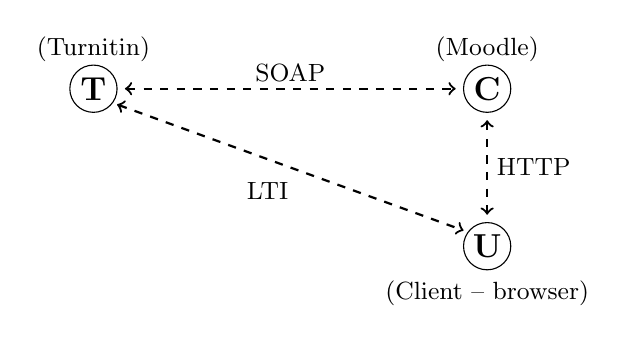
\begin{tikzpicture}
\draw (0,3.5) node{\small(Turnitin)};
\draw (0,3) node {\large\textbf{T}} circle(0.3cm);
\draw[thick,dashed,<->] (0.4,3) -- (4.6,3);
\draw (2.5,3.2) node{\small SOAP };
\draw (5,3.5) node {\small(Moodle)};
\draw (5,3) node {\large\textbf{C}} circle(0.3cm);
\draw[thick,dashed,<->] (5,2.6) --(5,1.4);
\draw (5.0,2) node[right]{\small HTTP};
\draw (5,1) node {\large\textbf{U}} circle(0.3cm);
\draw (5,0.4) node{\small(Client -- browser)};
\draw[thick,dashed,<->] (0.3,2.8) -- (4.7,1.2);
\draw (2.6,1.7) node[left] {\small LTI};

\end{tikzpicture}\end{center} \kern -14pt
\caption{Components and information flow}\label{fig:model}
\end{figure}
A typical user $U$ is a real person using a web browser
on a desktop computer or on a hand-held device. We use $U$ to note both
the browser and the person behind the interface.

The communication between the tool consumer $C$ and the service provider $T$
uses the SOAP protocol \cite{soap}. Requests and responses are well-formed
XML messages defined in several WSDL files \cite{wsdl}. The user $U$
is a 
web browser communicating with $C$ using the standard HTTP protocol. $U$ can
connect directly to $T$ using LTI calls over another HTTP or (preferably) HTTPS
connection. Such connections are initiated by
snippets embedded into the HTML code sent by $C$ to $U$. According to the IMS
recommendation, these LTI calls are \verb|POST| requests.

\subsubsection*{Remark}
The only way the client web browser can forward a \verb|POST| request is 
using a \verb|<form>| tag in the HTML code.
%%%%%%%%%%%%%%%%%
%% Lehet POST requestet csinalni AJAX request-kent is JavaScriptbol, pl. "type" a http://api.jquery.com/jQuery.ajax/ oldalon.
%% Amit nem lehet csinalni (vagy legalabbis nem latom, hogyan) az az, hogy egy IFRAMEt definialjunk, ami a tartalmat
%% POST-on keresztul toltene be, mert az IFRAMEnek egy URI kell.
%%%%%%%%%%%%%%%%%
To complete the forwarding,
either a user intervention is necessary (``push the submit button''), or 
running JavaScript should be permitted in the client browser.
\verb|GET| requests, however, can be redirected transparently, making a
conceptually cleaner (and simpler) solution.

Interestingly, Turnitin's response to such \verb|POST| LTI calls are 
redirects. Rather than letting $U$ send the LTI request, $C$ can send it on
behalf of $U$, capture the redirect, and send the redirect command to $U$,
which can then get the requested resource from $T$ without any extra user
intervention or running any JavaScript.

\section{Turnitin and LMS terminology}\label{sec:terminology}
The standard for Learning Management System (LMS) created its own terminology.
This table contains commonly used concepts roughly corresponding to LMS terms.
\begin{center}\begin{tabular}{|ll|}
\hline
\rule{0pt}{12pt}Turnitin & LMS \\
\hline
\rule{0pt}{11pt}course & context \\
class      & courseSection \\
assignment & lineItem      \\
submission & result        \\
student    & Learner       \\
teacher    & Instructor    \\
primary id & consumer key  \\
shared key & shared secret \\
\hline
\end{tabular}\end{center} 

\section{Security, authorization, authenticity}\label{sec:security}
Security is an intricate issue. Serious flaws are frequently discovered in systems used
by millions of users after several years of wide deployment. To avoid such problems, security
measures should be designed carefully, and with expertise. Unfortunately, it seems that in the
LMS standard security did not get the necessary attention; rather,
solutions routinely used by other companies were accepted seemingly without proper evaluation.

Traditionally, Tool Providers talk to Tool Consumers using secure connections
(HTTPS), and both parties are interested in keeping the joint secret,
which is used to authenticate requests and responses, under tight control.
Time stamps and randomly
set nonces prevent replay attacks, where the malicious party attempts to
re-send a previous request or response. Hashing messages with the join secret
achieves {\it integrity}, which means that messages cannot be altered
``en route'' by anyone controlling the transmission line. However, ensuring integrity
is unnecessary if the connection is already secure, as the
secure channel automatically guarantees this property. Rather, the sole role 
of the joint secret is to {\it authenticate} the message, ensuring for both 
parties that the messages are coming from someone who knows the secret.

Using an authentication method which does not require transmitting the join
secret (even over a secure channel) is preferred, as it could thwart attacks
against the channel (and not, in particular, against the security
of the message exchange). Security mechanisms used in the legacy Turnitin
API achieved the necessary security requirements in this way.

The situation is entirely different when LTI services are used. The Tool
Consumer $C$ {\it delegates} its authenticity to a third, typically
untrusted party, $U$, who, using the delegated credentials, approaches the
Tool Provider $T$ to get the granted services.
The {\it digital ticket}
which contains these credentials, should satisfy different, and more
stringent security measures. Some of the main differences are:
\begin{itemize}
\item The client $U$ is not interested in keeping the credentials secret.
\item The client $U$ cannot be assumed to be honest, as the client might
try to extract as much information from the ticket as possible.
\item While with timestamps and nonces, it can be ensured that the ticket can be used only once,
and for a limited time only, there is no time limit on {\it breaking 
the security of the ticket}.
\end{itemize}
Authenticity of the delegated tickets are ensured by the OAuth 1.0
authentication mechanism \cite{oauth1}, which digitally signs the
text of the ticket using the common secret shared by $C$ and $T$ as the key.
The ticket cannot be assumed to remain within a controllable environment,
thus mounting a dictionary attack {\it to find the signing key} is
a very probable scenario. This attack would be able to find the {\it common
secret}, and thus would let the attacker use all sources that $C$ is entitled
to use.

\subsubsection*{A possible scenario for exploiting the flaw}

In a LMS, a student has to upload her paper using a delegated ``submission
form''. The student then may capture the packet (simply by using the ``View document
source'' feature, or using web developer tools to investigate the document structure). Using
the data there, she can mount an attack to find out the shared secret. She
has unlimied time to succeed, and once she
recovered the secret key, she could pretend to be her teacher, give and
modify grades, look at materials prepared but not to be shown to students,
upload late submissions, etc.


\subsubsection*{Countermeasures to prevent the attack}

There are several possible countermeasures to prevent this kind of attack. One possibility
is to use {\it temporary keys} to sign tickets; temporary keys are 
negotiated by $C$ and $T$ and have a tight expiration date. Another
possibility is to make sure that the common secret has high entropy, thus it
cannot be guessed easily. 

To have a temporary remedy until a satisfactory solution is reached,
{\bf it would be advisable} if the common secret was generated by the Tool
Provider (and not the Tool Consumer), and was a long (at least 40 hexadecimal
digits) random number.


\section{Sample LTI calls}\label{sec:lti-calls}

All LTI calls go to the URI starting with \gt{https://HOSTNAME/api/lti/1p0};
the ending is
defined below. The requests are composed by the Tool Consumer $C$, and are
intended for submission to the Tool Provider $P$ by the web
browser $U$.
The LTI calls are authenticated using a method inherited from
the {\rm SOAP} authentication, and should use the POST method.

The following
parameters together with the request-specific parameters should be set and
sent with the request:

\args(lti\_message\_type,should be \gt{basic-lti-launch-request}, but seems
to be ignored by Turnitin)
\args(lti\_version,the version number; this is ``\gt{LTI-1p0}'')
\args(lang,for example, ``\gt{en\_us}'')
\args(resource\_link\_id,a random hex number identifying the request, see below;)
\args(custom\_source,the Turnitin integration code, presently this is {\tt
12}.)

\noindent
The \gt{resource\_link\_id} is a 8+4+4+4+12 hexadecimal digit-long random value;
the parts are separated by hyphens (\gt{-}). In the Moodle integration, 
five bits of this 128-bit random string are fixed: The first digit of the
third number is 4, and the first digit of the fourth number is 8 or bigger. 

\smallskip\noindent
The following parameters, while defined in the LTI standard, seem to be 
ignored:

\args(launch\_presentation\_return\_url,the full URL where the control returns
when the service is over)
\args(launch\_presentation\_css\_url,the full URL of a CSS resource to be included.)


\noindent
Parameters of the OAuth authentication:

\args(oauth\_version,it should be {\tt 1.0})
\args(oauth\_nonce,40 hexadecimal digits; a unique number)
\args(oauth\_timestamp,the standard unix time in seconds)
\args(oauth\_consumer\_key,the integration number supplied by Turnitin)
\args(oauth\_signature\_method,it should be ``\gt{HMAC-SHA1}'')
\args(oauth\_signature,the URL-encoded signature of all arguments of the
request.)

\subsubsection*{Remark on the number of random bits}
One can argue that there is too much ``randomness'' involved in the message. It is encoded
in the \gt{oauth\_nonce} and in the \gt{resource\_link\_id} fields. Their
lengths are 160 and 128 bits, respectively. For correct functioning, only the
{\it uniqueness} of these values is necessary over a reasonable period of time
(say, one day). Using only 32 random
bits, both fields could be padded with fixed values without loosing any
security.

\subsubsection*{Sample Turnitin LTI calls}

\begin{enumerate}
\item {\it Show a submission}

There are four calls in this group: the first one opens the submission page,
where there are three tabs: report, peermark, grademark. The other three
calls automatically open a specific tab.

Endpoints: \gt{/dv/default}, \gt{/dv/report}, \gt{/dv/peermark},
\gt{/dv/grademark}.

Arguments:

\args(lis\_person\_sourcedid,the viewer)
\args(roles,either Instructor or Learner)
\args(lis\_result\_sourcedid,the submission ID)

\item {\it Messages, rubric manager, quickmark}

View messages, use rubric or quickmark

Endpoints: \gt{/user/messages}, \gt{/user/rubric}, \gt{/user/quickmark}.

Arguments:

\args(lis\_person\_sourcedid,the user's ID)
\args(roles,either Instructor or Learner)

\item{\it Upload a document for similarity checking}

A document can be uploaded as a new request, or as a replacement for an
earlier submission. In the latter case it is accepted only if the assignment is
configured to allow resubmissions. When ``\gt{custom\_xmlresponse}'' is
set to 1, an XML response is sent back containing the assignment ID, and an
extract of the submitted document. The {\it content} of the uploaded 
document goes under the parameter name ``\gt{custom\_submission\_data}.''
When generating the OAuth signature, this parameter {\it should
not be included} in the computation. This means that the content of the
uploaded data is not authenticated; and the signature allows
whoever has access to the ticket to upload any
content for a given student {\it X}, under the title {\it Y}, and
assignment {\it Z}.

Endpoints: \gt{/upload/submit}, \gt{/upload/resubmit}.

Arguments:

\args(lis\_person\_sourcedid,the submitter's ID)
\args(roles,either the ``\gt{Instructor}'' or the ``\gt{Learner}'')
\args(custom\_submission\_title,the title of the paper, maximum 100 characters)
\args(custom\_submission\_author,the paper's author. The author {\it must} be
 enrolled in the class which contains this submission)
\args(custom\_xmlresponse,either 0 or 1, according to whether an XML response is
requested)
\args(lis\_lineitem\_sourcedid,the ID of the
assignment, only when submitting a new request)
\args(lis\_result\_sourcedid,the ID of the previous
submission to be replaced, only when resubmitting)
\args(custom\_submission\_data,the document to be submitted for similarity checking.)

When \gt{custom\_xmlresponse=1} is used, the returned XML response
contains the submission ID under
\gt{lis\_result\_sourcedid}.

\item{\it End User License Agreement} (EULA)

The user can accept the Turnitin's EULA on this form. 

Endpoint: \gt{/user/eula}.

Argument:

\args(lis\_person\_sourcedid,the ID of the person who will accept the
EULA.)

\end{enumerate}

\section{SOAP calls}\label{sec:soap-calls}
SOAP calls are used for direct communication between the Tool Provider and
Tool Consumer. The messages are well-formed XML sent and received
via HTTPS with appropriately set headers. The XML for requests
and responses is defined by WSDL resources defined in \cite{wsdl}. In the
examples below only the relevant arguments are indicated. Requests are 
sent to \gt{https://HOSTNAME/api/\allowbreak soap/\allowbreak
1p0/lis-<service>}, where \gt{<service>} is one of
\gt{result}, \gt{person}, \gt{membership}, \gt{coursesection},
and \gt{lineitem}. The XML reply should be parsed; the head
contains information about success or failure, and the body contains the
requested data.



The header of the HTTPS \verb|POST| request should contain the following:

\args(Content-type: text/xml; charset="utf-8",)
\args(Accept: text/xml,)
\args(SOAPAction: "http://<soap action>",the URL of the soap action)
\args(Content-length:, the length of the request data)
\args(Source: 12,Turnitin integration code)
\args(Authorization: OAuth <authorization data>,)
%%%% ^ Jo helyen van a vesszo?
\args(Cache-Control: no-cache,)

\medskip

As an example, the full xml request for retrieving a person's full record with 
record number \gt{22222222} is like the one shown here.
{\small\begin{verbatim}
<SOAP-ENV:Envelope 
   xmlns:SOAP-ENV="http://schemas.xmlsoap.org/soap/envelope/" 
   xmlns:ns1="http://www.imsglobal.org/services/lis/
                                      pms2p0/wsdl11/sync/imspms_v2p0">
 <SOAP-ENV:Header><ns1:imsx_syncRequestHeaderInfo>
    <ns1:imsx_version>V1.0</ns1:imsx_version>
    <ns1:imsx_messageIdentifier>97d5792c-13c4-4641-8f7a-
                             ea6d43279a02</ns1:imsx_messageIdentifier>
 </ns1:imsx_syncRequestHeaderInfo></SOAP-ENV:Header>
 <SOAP-ENV:Body><ns1:readPersonRequest>
    <ns1:sourcedId>22222222</ns1:sourcedId>
 </ns1:readPersonRequest></SOAP-ENV:Body>
</SOAP-ENV:Envelope>
\end{verbatim}}
%%%% Lehet, a messageIdentifier-t is ki kellene cserleni, pl. 9999-99...

\subsubsection*{Sample SOAP calls}
The description below
%%%% ^ which description? specification?
indicates what data is required by the function, and it is
not indicated under which XML node
%%%% ^ in the tree? under which node?
should it be inserted in the complete XML
request. This task can be done easily by inspecting the official WSDL
specification \cite{wsdl}.
%%%% ^ specification? Is it Turnitin-specific?

\begin{enumerate}
\item {\it Create a record for a person}

A new record for a person is created, if it does not exists. Supplied data:

\args(person,the service to be called)
\args(createByProxyPerson,the function)
\args(email,the primary e-mail address; this is used to uniquely identify the person)
\args(firstname,first and middle names)
\args(lastname,last name)
\args(role,Instructor, Learner, Admin, etc.)

The returned record is either empty, or, if the record has been created
successfully, it contains the record number (\gt{sourcedId}).

\item {\it Get a full record of a person}

The returned XML record contains all data stored under a specific person's
record number.

\args(person,the service to be called)
\args(readPerson,the function)
\args(personid,argument, the record number, the \gt{sourcedId}.)

\item {\it Find persons based on e-mail address}

This call returns all personal record IDs where the primary e-mail address
matches the given e-mail address.

\args(person,the service to be called)
\args(discoverPersonIds,the function)
\args(email,the email address to search for)


The search is successful even if there is no match.

\item {\it Create a class}

Classes are called ``course section''s in LMS. Only the course title is
necessary to create the class.

\args(coursesection,the service to be called)
\args(createByProxyCourseSection,the function)
\args(title,the title of the course)

The returned record contains the ID of the new course.

\item {\it Enroll a student in a class}

Only enrolled students are allowed to submit papers; thus students should be
enrolled into classes.

\args(membership,the service to be called)
\args(createByProxyMemembership,the function)
\args(classid,the ID of the class)
\args(personid,the ID of the person to be enrolled)
\args(role,either Instructor or Learner, the person's role)

The returned record contains the ID of a {\it membership} record which
connects the class and the person. One can search membership records containing a
certain person to get all things the person belongs to.

\item {\it Create an assignment}

Assignments are dubbed as ``line items''. Every assignment has a label, a
corresponding class, and three dates: start, due, and feedback. Several
custom parameters should be set as well, such as whether late submission is
allowed, whether every submission is final or resubmission is allowed, what is the
scale of grading, etc. Only a sample subset of possibilities are shown here.

\args(lineitem,the service to be called)
\args(createByProxyLineItem,the function)
\args(classid,the ID of the class this assignment belongs to)
\args(title,the title of the assignment)
\args(startdate,when the assignment starts accepting submissions)
\args(duedate,closing date)
\args(feedbacdate,when the grades are revealed to the students)
\args(LateSubmissionAllowed,yes or no)
\args(MaxGrade,the value of the maximum grade for this assignment)
\args(AnonymousMarking,yes or no, whether the name of submitter
should be shown or not, etc.)

The returned record contains the ID of the newly created lineItem (i.e., the
assignment).

\item {\it Obtain the score of a submitted paper}

After uploading a paper to an assignment, a ``result ID'' is returned. Also,
using a search (``discover'') function, the ID's of all submissions in an
assignment can be retrieved.


\args(result,the service to be called)
\args(readResult,the function)
\args(paperid,the ID of the submission -- typically a  result ID.)

The XML record returned contains the total score and its breakdown to sub-scores
depending on sources, the title, the author's ID, etc.

\end{enumerate}


\begin{thebibliography}{9}

\bibitem{oauth1}
The OAuth 1.0 Protocol (RFC 5849), \hfill\hbox{}
{\tt http://tools.ietf.org/html/rfc5849}

\bibitem{lti2} John Tibbetts,
{\it lti2 introduction}, \hfill\hbox{}
{\tt http://developers.imsglobal.org/tutorials.html}

\bibitem{moodlev2} John McGettrick,
Turnitin Moodle Direct version 2, \hfill\hbox{}
{\tt https://github.com/jmcgettrick/MoodleDirectV2}

\bibitem{soap}
{\it SOAP Specifications} -- World Wide Web Consortium, \hfill\hbox{}
{\tt http://www.w3.org/TR/}

\bibitem{wsdl}
IMS Global Learning Consortium, {\it Learning Information
Services},\hfill\hbox{}
{\tt http://www.imsglobal.org/lis/}

\bibitem{tutorial}
{\tt https://www.edu-apps.org/code.html}

\end{thebibliography}


\end{document}